\section{Sucção} % (fold)
\label{sub:aspirador}
	
	O sistema de sucção tem a função de aspirar pequenas partículas de sujeira e restos de alimentos pequenos. Para tal objetivo, será construída uma bomba de ar que irá gerar uma diferença de pressão entre o exterior e o interior do sistema, fazendo com que se induza um fluxo de ar para dentro do sistema. Esse fluxo de ar precisará ter intensidade suficiente para puxar as partículas desejadas. 

	Dois modelos básicos foram estudados. Um deles utiliza hélices controladas por motores elétricos que induzem uma diferença de pressão pela quantidade de vazão de ar que o sistema pode expulsar.  Um filtro é colocado para proteger o sistema de hélice e motor e para garantir o armazenamento das partículas aspiradas.

	O outro modelo é chamado de ciclone, utilizando o mesmo princípio para gerar diferença de pressão. Esse modelo não necessita de um filtro, pois o ar é sugado em uma trajetória helicoidal em torno de um cone, gerando um efeito de força centrípeta que leva a poeira até as paredes do aspirador. Uma vez nas paredes, a poeira começa a se depositar na parte inferior do cone, enquanto o ar escapa pela parte superior do cone \cite{layton}.

	\subsection{Solução} % (fold)
	\label{sub:solução}
		
		Para o projeto foi escolhido o primeiro modelo do ventilador com filtro, pois é uma solução com um custo menor e de fácil implementação se comparado ao sistema ciclone. Serão integradas nesse sistema escovas abaixo da linha de sucção, conhecidas como vassouras mágicas, que irão facilitar o transporte e direcionar a poeira para dentro do aspirador. Serão escolhidos dois coolers comerciais com uma vazão de ar por volta de 160 $m^3/h$, que serão colocados lado a lado dentro de um sistema hermeticamente fechado. 

		A geometria do sistema busca diminuir a área de escoamento na ponta da sucção para aumentar a velocidade do fluído na entrada, utilizando o princípio de conservação do fluxo de massa do sistema. O sistema de vedação será construído utilizando acrílico colado e mangueiras sanfonadas. Também será utilizado um motor para o acionamento da escova. Para o armazenamento do pó, será projetada uma caixa retangular de plástico com tampa. No momento da limpeza do depositório, o proprietário do aspirado deve apenas desencaixar a parte móvel, retirar as impurezas e encaixar novamente na tampa.

		Os dados relativos ao fluxo de massa e potência dos coolers comerciais é muito limitado. Assim o dimensionamento do sistema será realizado utilizando uma simulação de base no Ansys em conjunto com experimentos empíricos em protótipos simplificados. Para primeira análise, foi realizada uma simulação com as condições de contorno definidas pelo fluxo de massa constante na entrada e na saída, com um valor de 0,026Kg/s, dados fornecidos por fabricantes de coolers. A simulação mostrou uma velocidade de saída do escoamento de 5 m/s e a velocidade de entrada do ar de 19 m/s.

		A analise do fluxo de massa realizada no software \textit{Ansys} está apresentada na Figura \ref{img:analise_fluxo}.

		\begin{figure}[H]
			\centering
			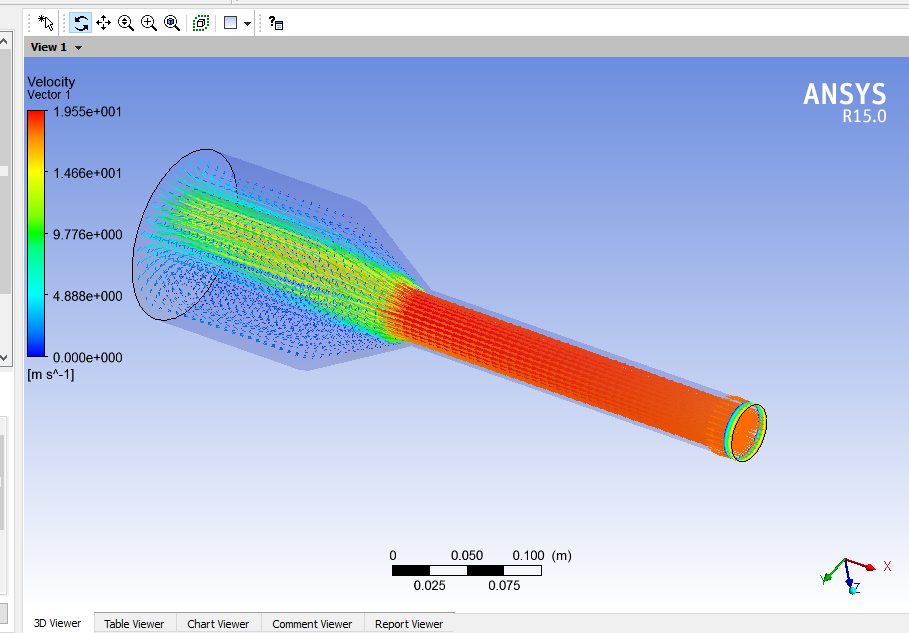
\includegraphics[scale=0.4]{figuras/analise_fluxo.png}
			\caption{Simulação do Ansys com o fluxo de massa de um cooler comercial.}
			\label{img:analise_fluxo}
		\end{figure}



	% subsection solução (end)
% section aspirador (end)